\section{Related Work}

Nat�rlich sind wir nicht die Ersten, die mit einer Kombination aus realer und virtueller Welt experimentieren. Es gibt schon einige etablierte Spiele, die beides erfolgreich verbindet. Aber auch in anderen Bereichen, wie der Medizin \cite{med} oder der Industrie, wird �ber die erweiterte Realit�t geforscht. 
H�ufig wird es im Sinne von viralem Marketing zur Bewerbung eines neuen Produktes oder einer neuen Dienstleistung verwendet, ohne dieses direkt anzupreisen und ohne das Spiel als Werbeveranstaltung erkennen zu lassen.
Im folgenden Abschnitt werden Spiele, die sich schon bewertet haben, kurz erleutert.

\subsubsection{Ingress}
Auch Google selbst l�sst sich nicht lumpen und hat ein erfolgreiches Spiel implementiert. Ingress \cite{ingress} ist ein kooperatives interaktives Gesellschaftsspiel, welches sich auf der ganzen Welt abspielt. Zu Anfang w�hlt ein Spieler eine von zwei Seiten. Von nun an geht es darum, mit seinem Team m�glichst gro�e �ffentliche Bereiche unter seine virtuelle Kontrolle zu bekommen. Wesentlicher Spielbestandteil ist der so genannte Scanner, die App des Spiels.

\begin{figure}[htbp]
  \centering
    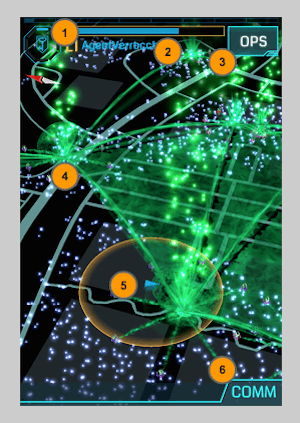
\includegraphics[width=0.5\textwidth]{2-Spielideen/2-3-Related_Work/ingress.png}
     \caption{der Scanner des Spiels Ingress. Auf der Karte werden "`Portale"' angezeigt und mit ihm k�nnen die Spieler untereinander agieren.
	(	Quelle: \url{https://lh3.ggpht.com/OC9nlsdM9HjIUMJ4BHpUtLArV5qXyyqphqMHUjsmXp82rYcmSJgcp4v5DmXI5R7eB2z1fckH=w300})
		}
\end{figure}


\subsubsection{Pacman auf Google-maps}

Ein weiteres kleines Minispiel, welches sich Google hat einfallen lassen, lies sich nur eine bestimme Zeit lang spielen. Um den 1. April 2015 konnte man auf der normalen Google-Maps Seite die Stra�enkarte in ein Pacman-Spiel \cite{pacman} verwandeln und sich somit durch seine eigene Stadt mit dem kleinen gelben Kreis fressen.

\begin{figure}[htbp]
  \centering
    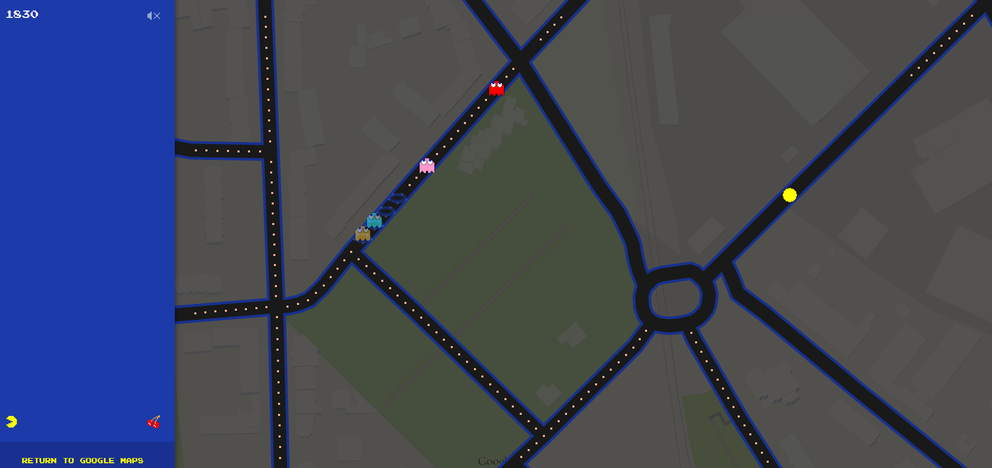
\includegraphics[width=0.9\textwidth]{2-Spielideen/2-3-Related_Work/pacman.png}
     \caption{Pacman auf Googlemaps
	(	Quelle: \url{http://media2.giga.de/2015/03/pacman-google-maps-rcm992x0.png})
		}
\end{figure}


\subsubsection{Twinkomplex}

Eine andere Idee hatte der Gr�nder von TwinKomplex. \cite{twinkomplex} Er l�sst den Spieler in die Rolle eines Agenten schl�pfen. Diese werden dann, durch Google-Maps und andere Open-Source Daten, durch echte Schaupl�tze gef�hrt um ihre F�lle zu l�sen. Hier wurde somit die reale Welt in ein virtuelles Spiel �berf�hrt.

\begin{figure}[htbp]
  \centering
    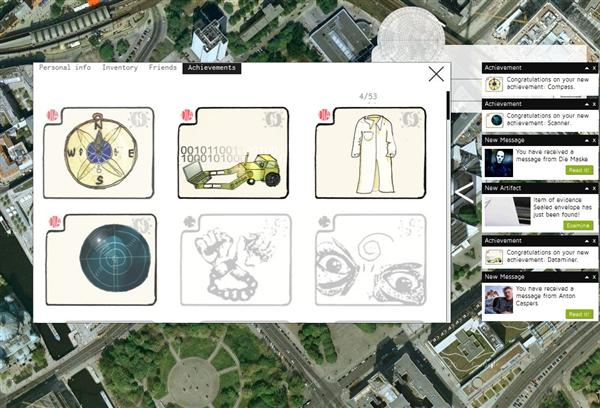
\includegraphics[width=0.65\textwidth]{2-Spielideen/2-3-Related_Work/twinkomplex.png}
     \caption{Screenshot des Spiels TwinKomplex
		Quelle: (\url{http://www.onlinegameslist.org/wp-content/uploads/2012/01/twinkomplex-game-achievements.jpg})
		}
\end{figure}
